% MORPH — Attention Detail (triple-axis compression: CCA x {CSA|HCA} x window).
% The zoom-in of the "CCA + CSA/HCA Attention" box in morph_block.tex.
% LAYOUT: horizontal CCA prologue "subway" strip along the bottom (the shared
% channel-compress front-end), feeding a vertical branch/combine fork above it.
% Detail lives in EXACTLY one place (no summary-box + inset duplication).
%
% Verified against code (2026-06-07, morph/model/attention.py + transformer.py:322-354):
%   - _CCABase shared prologue: W_down_q 768->384, W_down_k 768->128 (C=2, d_head=32);
%     depthwise+head-grouped causal conv (k=4); QK-mean couple; QK-RMSNorm; key temp
%     exp() (per kv head); CoPE (clipped-RoPE); GQA expand 4->12; value-shift.
%   - Window branch (always): sliding causal, w=128, XSA (self excluded), fused.
%   - Global-compressed slot resolved at __init__ by GLOBAL layer_idx parity:
%       even -> CSA: two-stream pool m=4 -> Lightning Indexer (-inf before relu)
%               -> top_k=128 select -> on-the-fly gather + invalid-mask -> flash.
%       odd  -> HCA: single-stream pool m=128 -> DENSE attn over all blocks + early-q guard.
%   - Combine: per-head sigmoid gate (2 wts/head) blends; + residual-alpha (q_lat);
%     + learnable per-head sinks; W_up 384->768.  CLA = dashed optional (default off).
% Compile: pdflatex morph_attention.tex

\documentclass[border=14pt]{standalone}
\usepackage[T1]{fontenc}
\usepackage{amsmath,amssymb}
\usepackage{tikz}
\usetikzlibrary{arrows.meta, fit, positioning, calc, backgrounds, decorations.pathreplacing}

% ── Palette (Paul Tol, colorblind-safe — matches the figure family) ───────────
\definecolor{cbBlue}{HTML}{4477AA}
\definecolor{cbOrange}{HTML}{EE7733}
\definecolor{cbPurple}{HTML}{AA3377}
\definecolor{cbTeal}{HTML}{228833}
\definecolor{cbGray}{HTML}{777777}
\definecolor{fBlue}{HTML}{DCEAF7}
\definecolor{fOrange}{HTML}{FDE8D0}
\definecolor{fPurple}{HTML}{EEDCEE}
\definecolor{fTeal}{HTML}{D6EFDD}
\definecolor{fGray}{HTML}{EBEBEB}
\definecolor{bdr}{HTML}{555555}
\definecolor{ccaC}{HTML}{2255AA}

\tikzset{
  % strip step (CCA prologue subway)
  sb/.style={draw=cbBlue!70, rounded corners=3pt, fill=fBlue!60,
    minimum width=2.45cm, minimum height=1.05cm,
    font=\scriptsize\sffamily, align=center, inner sep=2pt},
  % branch / combine boxes
  Bx/.style={draw=bdr, thick, rounded corners=4pt,
    minimum width=3.4cm, minimum height=1.0cm,
    font=\small\sffamily, align=center, inner sep=4pt},
  % small box inside the global slot
  gs/.style={draw=bdr, rounded corners=3pt, minimum width=2.5cm,
    minimum height=0.66cm, font=\scriptsize\sffamily, align=center, inner sep=2pt},
  io/.style={font=\small\sffamily},
  A/.style={-{Stealth[length=2.8mm,width=2.2mm]}, thick},
  As/.style={-{Stealth[length=2.4mm,width=1.9mm]}, semithick},
  Ad/.style={-{Stealth[length=2.4mm,width=1.9mm]}, thick, densely dashed},
  rail/.style={ccaC, line width=1.4pt},
  sub/.style={font=\scriptsize\sffamily},
  tny/.style={font=\tiny\sffamily},
  dim/.style={font=\tiny\sffamily, text=cbGray},
}

\begin{document}
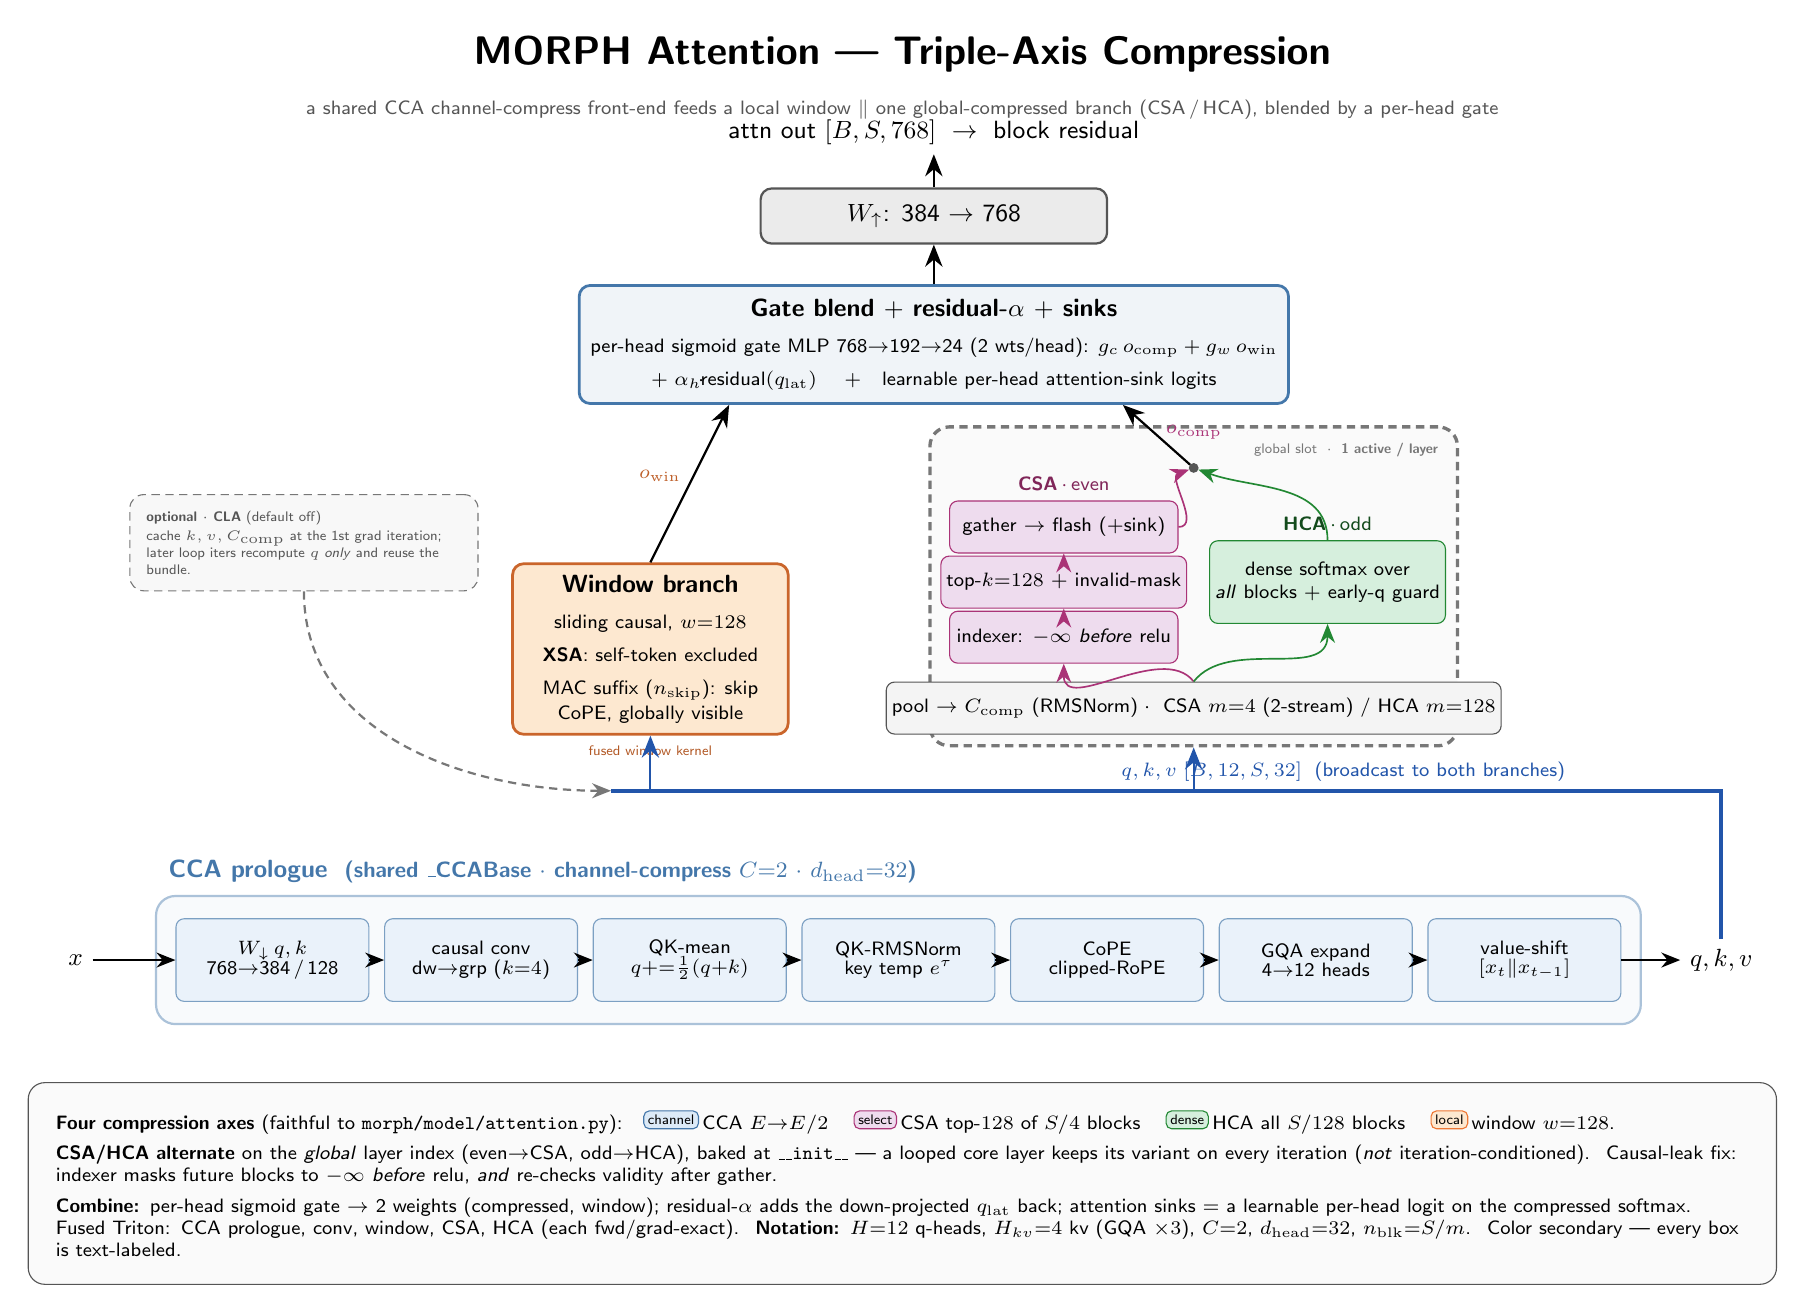
\begin{tikzpicture}

% =====================================================================
% BAND 1 (bottom) — CCA prologue subway strip
% =====================================================================
\def\sy{0.3}
\node[io] (xin) at (-10.5,\sy) {$x$};
\node[sb] (s1) at (-8.0,\sy) {$W_{\downarrow}\,q,k$\\[-1pt]768$\to$384\,/\,128};
\node[sb] (s2) at (-5.35,\sy) {causal conv\\[-1pt]dw$\to$grp ($k{=}4$)};
\node[sb] (s3) at (-2.70,\sy) {QK-mean\\[-1pt]$q{+}{=}\tfrac12(q{+}k)$};
\node[sb] (s4) at (-0.05,\sy) {QK-RMSNorm\\[-1pt]key temp $e^{\tau}$};
\node[sb] (s5) at (2.60,\sy) {CoPE\\[-1pt]clipped-RoPE};
\node[sb] (s6) at (5.25,\sy) {GQA expand\\[-1pt]4$\to$12 heads};
\node[sb] (s7) at (7.90,\sy) {value-shift\\[-1pt]$[x_t\Vert x_{t-1}]$};
\node[io] (qkv) at (10.4,\sy) {$q,k,v$};
\foreach \a/\b in {xin/s1,s1/s2,s2/s3,s3/s4,s4/s5,s5/s6,s6/s7,s7/qkv}{\draw[As] (\a)--(\b);}
\begin{scope}[on background layer]
  \node[draw=cbBlue!45, thick, rounded corners=7pt, fill=cbBlue!4,
        fit=(s1)(s7), inner xsep=7pt, inner ysep=8pt] (STRIP) {};
\end{scope}
\node[font=\small\sffamily\bfseries, text=cbBlue, anchor=south west]
  at ($(STRIP.north west)+(0.05,0.03)$)
  {CCA prologue \;{\footnotesize(shared \_CCABase $\cdot$ channel-compress $C{=}2$ $\cdot$ $d_\mathrm{head}{=}32$)}};

% =====================================================================
% q,k,v broadcast rail (compute once, feed both branches)
% =====================================================================
\def\busy{2.45}
\draw[rail] (qkv.north) |- (-3.7,\busy);
\node[sub, text=ccaC, anchor=south] at (5.6,\busy) {$q,k,v\;[B,12,S,32]$ \;(broadcast to both branches)};

% =====================================================================
% BAND 2 (middle) — two attention branches
% =====================================================================
% LEFT: window branch
\node[Bx, fill=fOrange, draw=cbOrange!85!black, line width=1pt,
      minimum width=3.5cm, minimum height=2.0cm, anchor=south] (win) at (-3.2,3.15) {
  \textbf{Window branch}\\[2pt]
  {\scriptsize sliding causal, $w{=}128$}\\[1pt]
  {\scriptsize \textbf{XSA}: self-token excluded}\\[1pt]
  {\scriptsize MAC suffix ($n_\mathrm{skip}$): skip}\\[-2pt]
  {\scriptsize CoPE, globally visible}};
\node[tny, text=cbOrange!75!black, anchor=north] at (win.south) {fused window kernel};

% RIGHT: global-compressed slot (the alternation container)
\node[draw=cbGray, densely dashed, very thick, rounded corners=7pt, fill=cbGray!4,
      minimum width=6.7cm, minimum height=4.05cm, anchor=south] (slot) at (3.7,3.0) {};
\node[tny, text=cbGray, anchor=north east] at ($(slot.north east)+(-0.14,-0.1)$)
  {global slot \;$\cdot$\; \textbf{1 active / layer}};
% shared pooler at the bottom
\node[gs, fill=fGray!55, minimum width=6.0cm] (pool) at (3.7,3.5) {
  pool $\to C_\mathrm{comp}$ (RMSNorm)\;$\cdot$\; CSA $m{=}4$ (2-stream) / HCA $m{=}128$};
% CSA column (left, EVEN layers) — purple
\node[gs, fill=fPurple, draw=cbPurple, minimum width=2.9cm] (csa1) at (2.05,4.40) {indexer: $-\infty$ \emph{before} relu};
\node[gs, fill=fPurple, draw=cbPurple, minimum width=2.9cm] (csa2) at (2.05,5.10) {top-$k{=}128$ $+$ invalid-mask};
\node[gs, fill=fPurple, draw=cbPurple, minimum width=2.9cm] (csa3) at (2.05,5.80) {gather $\to$ flash ($+$sink)};
\node[sub, text=cbPurple!75!black, anchor=south] at (csa3.north) {\textbf{CSA}\,$\cdot$\,even};
% HCA column (right, ODD layers) — green
\node[gs, fill=fTeal, draw=cbTeal, minimum width=2.9cm, minimum height=1.05cm] (hca) at (5.4,5.10)
  {dense softmax over\\ \emph{all} blocks $+$ early-q guard};
\node[sub, text=cbTeal!55!black, anchor=south] at (hca.north) {\textbf{HCA}\,$\cdot$\,odd};
% pool feeds both columns; csa flows up; both merge to ONE o_comp exit (only one runs/layer)
\draw[As, cbPurple] (pool.north) to[out=128,in=-90] (csa1.south);
\draw[As, cbTeal]   (pool.north) to[out=52,in=-90]  (hca.south);
\draw[As, cbPurple] (csa1) -- (csa2);
\draw[As, cbPurple] (csa2) -- (csa3);
\node[circle, draw=bdr, fill=bdr, inner sep=1.1pt] (mrg) at (3.7,6.55) {};
\draw[As, cbPurple] (csa3.east) to[out=0,in=200] (mrg);
\draw[As, cbTeal]   (hca.north) to[out=90,in=-20] (mrg);

% rail risers into the two branches
\draw[A, ccaC] (-3.2,\busy) -- (win.south);
\draw[A, ccaC] (3.7,\busy) -- (slot.south);

% =====================================================================
% BAND 3 (top) — combine + up-project + output
% =====================================================================
\node[Bx, fill=cbBlue!8, draw=cbBlue, line width=1pt, minimum width=8.4cm,
      minimum height=1.5cm, anchor=south] (comb) at (0.4,7.35) {
  \textbf{Gate blend $+$ residual-$\alpha$ $+$ sinks}\\[2pt]
  {\scriptsize per-head sigmoid gate MLP 768$\to$192$\to$24 (2 wts/head): $g_c\,o_\mathrm{comp}+g_w\,o_\mathrm{win}$}\\[1pt]
  {\scriptsize $+\;\alpha_h\!\cdot\!$residual$(q_\mathrm{lat})$ \quad$+$\quad learnable per-head attention-sink logits}};
\draw[A] (win.north) -- ([xshift=-2.6cm]comb.south)
  node[pos=0.55, left=1pt, sub, text=cbOrange!80!black]{$o_\mathrm{win}$};
\draw[A] (mrg) -- ([xshift=2.4cm]comb.south)
  node[pos=0.55, right=1pt, sub, text=cbPurple]{$o_\mathrm{comp}$};
\node[Bx, fill=fGray, minimum width=4.4cm, minimum height=0.7cm, above=0.5cm of comb] (wup)
  {$W_{\uparrow}$: 384 $\to$ 768};
\draw[A] (comb) -- (wup);
\node[io, above=0.42cm of wup] (out) {attn out $[B,S,768]$ \;$\to$\; block residual};
\draw[A] (wup) -- (out);

% ── CLA optional overlay (default off) — upper-left dead space ──
\node[draw=cbGray, densely dashed, rounded corners=5pt, fill=cbGray!5,
      text width=4.0cm, font=\tiny\sffamily, align=left, inner sep=6pt, text=bdr]
      at (-7.6,5.6) (cla) {%
  \textbf{optional $\cdot$ CLA} (default off)\\[1pt]
  cache $k,v,C_\mathrm{comp}$ at the 1st grad iteration; later loop iters recompute
  \emph{$q$ only} and reuse the bundle.};
\draw[Ad, cbGray] (cla.south) to[out=-90,in=180] (-3.7,\busy);

% =====================================================================
% BOTTOM — facts / notation panel
% =====================================================================
\node[draw=bdr, rounded corners=6pt, fill=fGray!25, inner sep=10pt,
      align=left, font=\scriptsize\sffamily, text width=21.5cm, anchor=north]
      (facts) at (0,-1.25) {%
  \textbf{Four compression axes} (faithful to \texttt{morph/model/attention.py}):\quad
  \tikz\node[draw=cbBlue,fill=fBlue,rounded corners=2pt,inner sep=1.5pt,font=\tiny\sffamily]{channel};\,CCA $E{\to}E/2$ \;\;
  \tikz\node[draw=cbPurple,fill=fPurple,rounded corners=2pt,inner sep=1.5pt,font=\tiny\sffamily]{select};\,CSA top-$128$ of $S/4$ blocks \;\;
  \tikz\node[draw=cbTeal,fill=fTeal,rounded corners=2pt,inner sep=1.5pt,font=\tiny\sffamily]{dense};\,HCA all $S/128$ blocks \;\;
  \tikz\node[draw=cbOrange,fill=fOrange,rounded corners=2pt,inner sep=1.5pt,font=\tiny\sffamily]{local};\,window $w{=}128$.\\[3pt]
  \textbf{CSA/HCA alternate} on the \emph{global} layer index (even$\to$CSA, odd$\to$HCA), baked at \texttt{\_\_init\_\_} —
  a looped core layer keeps its variant on every iteration (\emph{not} iteration-conditioned).
  \;Causal-leak fix: indexer masks future blocks to $-\infty$ \emph{before} relu, \emph{and} re-checks validity after gather.\\[3pt]
  \textbf{Combine:} per-head sigmoid gate $\to$ 2 weights (compressed, window); residual-$\alpha$ adds the down-projected $q_\mathrm{lat}$ back;
  attention sinks $=$ a learnable per-head logit on the compressed softmax. \;Fused Triton: CCA prologue, conv, window, CSA, HCA (each fwd/grad-exact).
  \;\textbf{Notation:} $H{=}12$ q-heads, $H_{kv}{=}4$ kv (GQA $\times3$), $C{=}2$, $d_\mathrm{head}{=}32$, $n_\mathrm{blk}{=}S/m$. \;Color secondary — every box is text-labeled.};

% ── Title ────────────────────────────────────────────────────────────
\node[font=\Large\sffamily\bfseries, anchor=south] (ttl) at (0,11.45)
  {MORPH Attention --- Triple-Axis Compression};
\node[sub, text=bdr, anchor=north, below=0.1cm of ttl]
  {a shared CCA channel-compress front-end feeds a local window $\Vert$ one global-compressed branch (CSA\,/\,HCA), blended by a per-head gate};

\end{tikzpicture}
\end{document}
